\documentclass[a4paper,14pt]{extarticle}
\pdfinfoomitdate=1
\pdftrailerid{}
\usepackage{thesis}
\usepackage{csquotes}
\usepackage[
  backend=biber,
  style=gost-numeric,
  language=auto,
  autolang=other,
  bibencoding=utf8,
  sorting=nyt
]{biblatex}
\addbibresource{references.bib}
\usepackage{euscript}
\usepackage{longtable}
\usepackage{makecell}
\usepackage[pdftex]{graphicx}
\usepackage{amsthm,amssymb, amsmath}
\usepackage{textcomp}
\usepackage{caption}
\usepackage{hyperref}
\usepackage{xcolor} % to access the named colour LightGray
\definecolor{LightGray}{gray}{0.9}
\usepackage[cache=false]{minted}
% \usepackage{newfloat}
\setminted[python]{%
  baselinestretch=1.2,
  bgcolor=LightGray,
  fontsize=\footnotesize,
  breaklines,
  linenos
}
\usepackage{caption}
\captionsetup[listing]{hypcap=false}
\begin{document}
\newgeometry{left=30mm, top=20mm, right=15mm, bottom=20mm, nohead, nofoot}
\begin{titlepage}
    \begin{center}
        \textbf{Санкт--Петербургский}
        \textbf{государственный университет}
        \vspace{35mm}\\
        \textbf{\textit{\large ТРЕТЬЯКОВ Даниил Александрович}} \\[8mm]
        \textbf{\large Выпускная квалификационная работа}\\[3mm]
        \textbf{\textit{\large Исследование эффективности непрерывного обучения с 
        использованием сетей Колмогорова-Арнольда в задаче распознавания образов}}
        \vspace{20mm}\\
        Уровень образования: бакалавриат\\
        Направление 01.03.02 «Прикладная математика и информатика»\\
        Основная образовательная программа СВ.5005.2021
        «Прикладная математика, фундаментальная информатика и
        программирование»\\[25mm]
        \begin{flushright}
            \begin{minipage}[t]{0.65\textwidth}
                {Научный руководитель:} \\
                профессор кафедры компьютерного моделирования и
                многопроцессорных систем, д.т.н. Дегтярев Александр Борисович
                \vspace{10mm}\\
                {Рецензент:} \\
                доцент кафедры компьютерного моделирования и многопроцессорных
                систем, к.ф.-м.н. Корхов Владимир Владиславович
            \end{minipage}
        \end{flushright}
        \vfill
        {Санкт-Петербург}
        \par{\the\year{} г.}
    \end{center}
\end{titlepage}
\restoregeometry
\addtocounter{page}{1}
\tableofcontents
\pagebreak




\specialsection{Введение}
В последние десятилетия нейронные сети стали одним из ключевых компонентов
современных интеллектуальных систем. Именно нейронные сети сделали возможным появление алгоритмов, превосходящих 
человеческие возможности в узкоспециализированных задачах, где люди традиционно
считались непревзойденными, например, в распознавании изображений и речи, играх
и стратегиях, медицинской диагностике.

Однако в отличие от человека, для нейронной сети, после того как она была
обучена выполнению определенной задачи, например, классификации деревьев,
обучение дополнительной задаче, например, классификации птиц, оказывается 
затруднительным. Это связано с тем, что при добавлении новой задачи типичная
нейронная сеть склонна «забывать» предыдущую. В связи с этим, одним из
актуальных направлений в развитии нейронных сетей является непрерывное обучение
- подход, при котором модель способна обучаться и адаптироваться на протяжении 
всего срока эксплуатации с целью поддержания своей производительности при
изменяющихся условиях окружающей среды и данных, без необходимости полного 
переобучения. Потребность в подобных моделях особенно сильна в рекламной
индустрии, финансовой аналитике, робототехнике и кибербезопасности.

Как правило, в исследованиях, посвященных методам преодоления катастрофического
забывания, рассматривается многослойный перцептрон\\ (Multi-Layer Perceptron,
MLP). Несмотря на то, что в борьбе с катастрофическим забыванием в многослойном
перцептроне были достигнуты определенные успехи, в последние месяцы растёт 
интерес к многообещающей альтернативе - нейронной сети Колмогорова-Арнольда (Kolmogorov-Arnold Network,
KAN), ключевые отличия которой представлены на рисунке \ref{fig:kan_vs_mlp}.
\begin{figure}[ht]
    \centering
    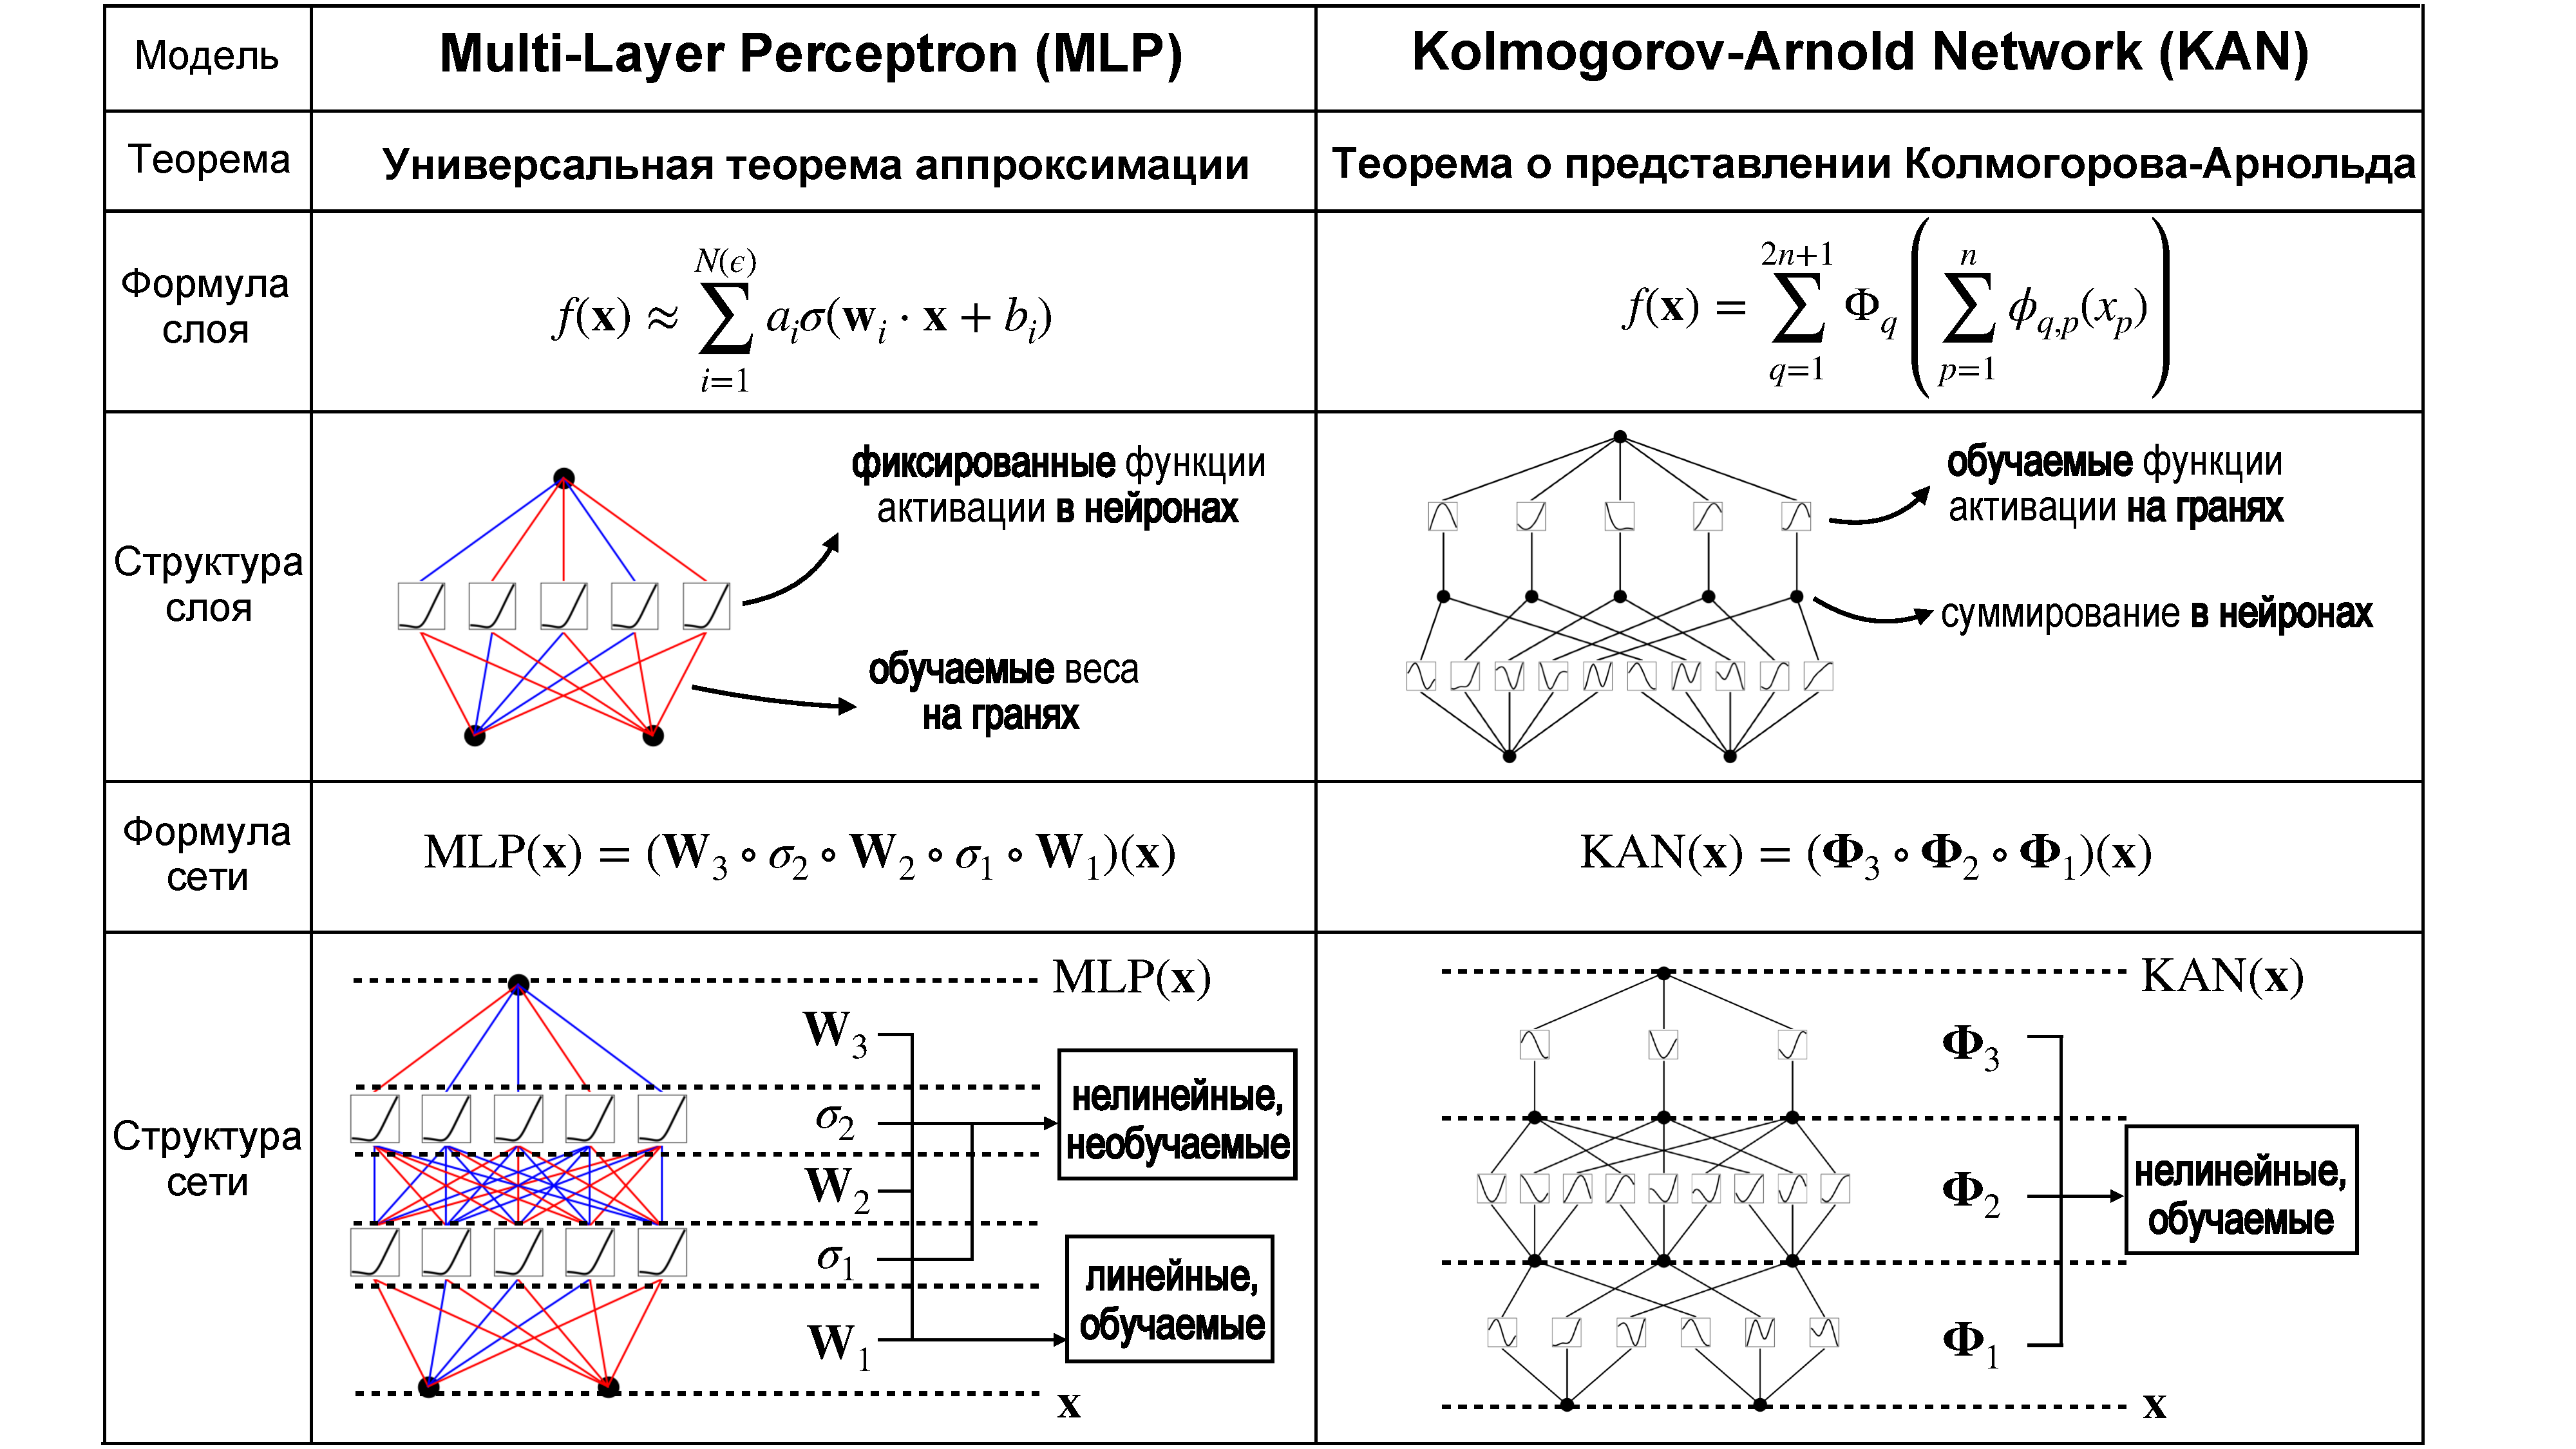
\includegraphics[width=\linewidth]{figures/kan_vs_mlp.pdf}
    \caption{Сравнение MLP и KAN. Адаптировано из \cite{liu2024kan},
        лицензия: CC BY 4.0.}
    \label{fig:kan_vs_mlp}
\end{figure}

Главная причина, по которой KAN представляет интерес с точки зрения применения в
условиях непрерывного обучения, заключается в возможности параметризации функции
активации таким образом, чтобы изменение параметров в одной области пространства
не влияло на другие области. Это возможно, например, при использовании 
B-сплайнов, обладающих локальной поддержкой. Поскольку обучение на новых данных
будет затрагивать лишь несколько соседних параметров, информация, сохранённая в
остальных параметрах, остается нетронутой. В MLP, напротив, даже отдельные
изменения могут повлиять на информацию, хранящуюся в отдалённых друг от друга
параметрах.

Для демонстрации преимуществ, связанных с локальной поддержкой функции
активации, предлагается рассмотреть простейшую задачу одномерной регрессии, 
детали которой приведены на рисунке \ref{fig:toy_cl_problem}: обучение состоит 
из 5 тренировочных сессий, в каждой из которых используются исключительно 
объекты из соответствующей части набора данных, также разделённого на 5 частей.
Можно заметить, что в данной задаче KAN изменяет только те параметры, которые 
отвечают за аппроксимацию зависимости в данных текущей тренировочной сессии, в
то время как MLP оказывается не способен сохранить информацию, полученную в
течение предыдущих тренировочных сессий.
\begin{figure}[ht]
    \centering
    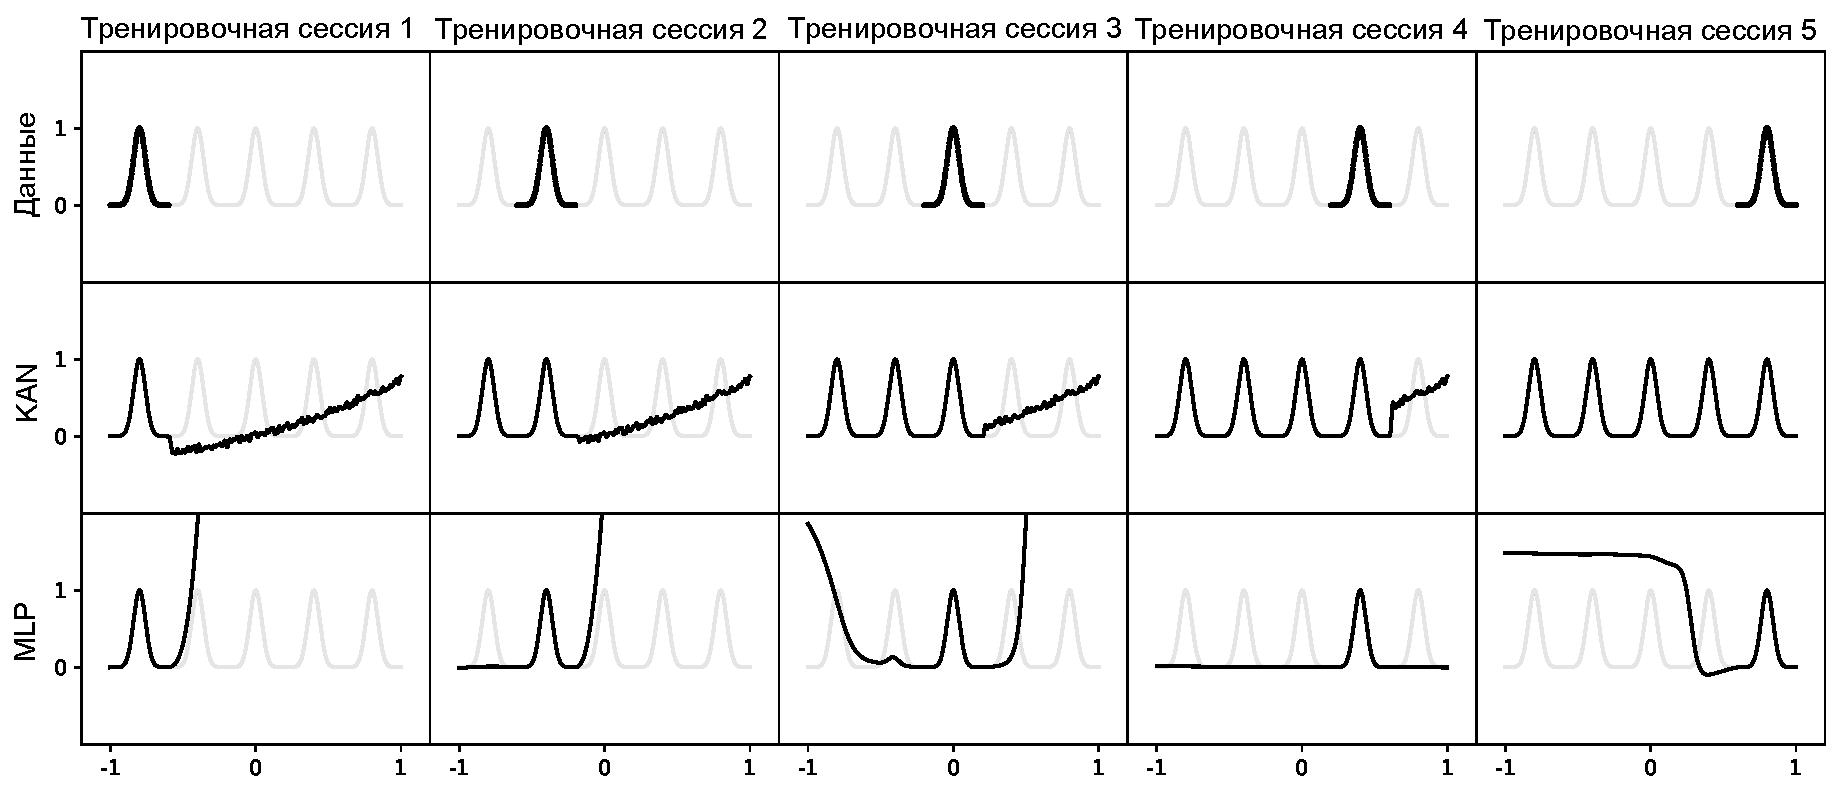
\includegraphics[width=\linewidth]{figures/toy_cl_problem.pdf}
    \caption{Простейшая задача непрерывного обучения: по горизонтали показаны 5
        последовательных тренировочных сессий одномерной регрессии
        («Тренировочная сессия 1-5»); по вертикали — три строки: «Данные»
        (данные, используемые в текущей тренировочной сессии, выделены чёрным,
        остальные серым), «KAN» (предсказания сети KAN) и «MLP» (предсказания
        сети MLP). Адаптировано из \cite{liu2024kan}, лицензия: CC BY 4.0.}
    \label{fig:toy_cl_problem}
\end{figure}
Рассмотренная задача является лишь упрощённым примером, в котором особенности
архитектуры KAN позволили существенно повлиять на эффективность непрерывного 
обучения. В прикладных задачах размерность параметрического пространства 
нейронных сетей, как правило, значительно выше, и сохранение свойства
локальности изменений параметров оказывается под вопросом.

Поскольку необходимым условием для достижения максимальной эффективности
непрерывного обучения является использование нейронных сетей в сочетании с
методами противодействия катастрофическому забыванию, тестирование оригинальной
архитектуры KAN без этих методов не позволит в полной мере оценить перспективы
её применения в непрерывном обучении. Поэтому главная цель данной работы -
адаптировать методы противодействия, разработанные для многослойного
перцептрона, для использования в сетях Колмогорова-Арнольда и выяснить,
позволяет ли локальная природа KAN упростить или усилить классические приёмы,
лежащие в основе этих методов. С этой целью эффективность полученных моделей
исследуется в условиях непрерывного обучения на задаче распознавания образов с
использованием набора данных CUB200, обладающего свойствами, характерными для
прикладных задач.

Полный исходный код, а также графические материалы, использованные в данной
работе, размещены в открытом репозитории на GitHub \cite{spbubachelorthesis}.
\pagebreak




\specialsection{Постановка задачи}
Рассматривается процесс непрерывного обучения в задаче многоклассовой
классификации в признаковом пространстве \(\mathcal{X}\subseteq\mathbb{R}^d\)
с множеством классов \(\mathcal{Y}=\{1,\dots,C\}\), где \(d\) - размерность
признакового пространства, \(C\) - число классов. Дана обучающая выборка \(D\),
состоящая из размеченных объектов, разбитых на \(T\) частей, соответствующих
тренировочным сессиям \(B_t\), то есть \(D=\{B_t\}_{t=1}^T\). Каждая
тренировочная сессия состоит из \(N_t\) объектов (\(N_t\) может изменяться между
сессиями). Таким образом, \(B_t=\{(x_i,y_i)\}_{i=1}^{N_t}\), где
\(x_i\in\mathcal{X},\,y_i\in\mathcal{Y}\). Предполагается, что элементы в каждой
тренировочной сессии независимы и имеют одинаковое совместное распределение
данных и меток классов \(\mathbb{D}_t,\,t=1,\dots,T\). Нейронная сеть 
\(f_\theta:\mathcal{X} \to \mathbb{R}^C\) с параметрами
\(\theta\in\mathbb{R}^{\left|\theta\right|}\) последовательно обучается решению
\(T\) задач, используя объекты текущей тренировочной сессии. Иначе говоря, в 
момент времени \(t\) модели предоставлены лишь данные из \(B_t\).

Требуется получить модель \(f_\theta\), способную сохранять информацию,
полученную в предыдущих тренировочных сессиях обучения, и одновременно
эффективно усваивать новые знания, приобретённые в течение последней
тренировочной сессии. Для оценки качества обучения модели в текущей
тренировочной сессии используется следующий функционал:
\begin{equation}
    Q(f_\theta,B_t)=\frac{1}{N_t}\sum_{(x,y)\in B_t}\mathcal{L}(f_\theta(x),y),
\end{equation}
где \(\mathcal{L}\) - кросс‑энтропийная функция потерь. Параметры модели 
\(\theta\) подбираются таким образом, чтобы минимизировать функционал \(Q\).
Обучение сводится к нахождению оптимальных параметров \(\theta_t\), которые
сохраняются после завершения текущей тренировочной сессии и используются в
качестве начальных значений в следующей:
\begin{equation}
    \theta_t=\arg\min_{\theta}Q(f_\theta,B_t)=\arg\min_{\theta}\frac{1}{N_t}\sum_{(x,y)\in B_t}\mathcal{L}(f_\theta(x),y),
\end{equation}

Для количественной оценки способности моделей противостоять катастрофическому
забыванию в процессе непрерывного обучения используются метрики, описанные в
\cite{kemker2017measuring}:
\begin{equation}
    \Omega_{base}=\frac{1}{T-1}\sum_{i=2}^{T}\frac{\alpha_{base,i}}{\alpha_{ideal}},
\end{equation}
\begin{equation}
    \Omega_{new}=\frac{1}{T-1}\sum_{i=2}^{T}\frac{\alpha_{new,i}}{\alpha_{ideal}},
\end{equation}
\begin{equation}
    \Omega_{all}=\frac{1}{T-1}\sum_{i=2}^{T}\frac{\alpha_{all,i}}{\alpha_{ideal}},
\end{equation}
где:\\
\(\alpha_{ideal}\) - значение метрики accuracy на совокупности всех тестовых
выборок \(D\), полученное при оффлайн обучении модели без механизмов
противодействия катастрофическому забыванию,\\
\(\alpha_{base,i}\) - значение метрики accuracy на тестовой выборке первой
тренировочной сессии после обучения модели в \(i\)-ой тренировочной
сессии,\\
\(\alpha_{new,i}\) - значение метрики accuracy на тестовой выборке \(i\)-ой
тренировочной сессии после обучения модели на этой же тренировочной сессии,\\
\(\alpha_{all,i}\) - значение метрики accuracy на совокупности тестовых выборок
всех предыдущих тренировочных сессий.

Таким образом, \(\Omega_{new}\) измеряет способность модели использовать только
что приобретенные знания, \(\Omega_{base}\) измеряет способность модели
удерживать в памяти знания, полученные в первой тренировочной сессии, а
\(\Omega_{all}\) оценивает общую эффективность использования накопленных знаний.
\subsection*{Цель и задачи исследования}
Целью данной работы является исследование эффективности применения архитектуры
KAN в сочетании с методами противодействия катастрофическому забыванию в задаче
распознавания образов в условиях непрерывного обучения. Для достижения
поставленной цели необходимо решить следующие задачи:
\begin{enumerate}
    \item Изучить методы противодействия катастрофическому забыванию,
        разработанные для многослойного перцептрона, и выделить основные
        подходы, лежащие в основе этих методов.
    \item Адаптировать для архитектуры KAN методы, использующие разные подходы,
        и разработать на их основе модифицированные модели.
    \item Применить оригинальную и модифицированные модели KAN в задаче
        распознавания образов в условиях непрерывного обучения с использованием
        набора данных CUB200.
    \item Сравнить противодействие катастрофическому забыванию между
        оригинальной и модифицированными моделями и выяснить, помогает ли
        свойство локальной поддержки функций активации KAN повысить
        эффективность классических приёмов, использованных в этих моделях.
    \item Проанализировать полученные результаты и оценить перспективы
        применения сетей Колмогорова-Арнольда в задачах непрерывного обучения.
\end{enumerate}
\pagebreak




\specialsection{Обзор литературы}
Нейронная сеть Колмогорова-Арнольда, составляющая основу данного исследования,
описана в статьях \cite{liu2024kan,liu2024kan2}, где вводятся архитектуры KAN и
MultKAN, позиционируемые в качестве альтернативы MLP. В \cite{liu2024kan}
поднимается вопрос о необходимости исследования потенциала сетей
Колмогорова-Арнольда в непрерывном обучении на задачах высокой размерности,
также в обеих статьях проводятся многочисленные эксперименты, демонстрирующие
интерпретируемость новых архитектур и их применимость в качестве инструмента
символьной регрессии. Всестороннее сравнение архитектур KAN и MLP представлено в
работе \cite{yu2024kan}. В ней делается вывод о том, что KAN демонстрирует
преимущество только в задаче символьной регрессии, а в остальных задачах
машинного обучения, включая задачи компьютерного зрения (Computer Vision, CV),
обработки естественного языка (Natural Language Processing, NLP) и обработки
аудиосигналов (audio processing), уступает. В частности, показано, что в
условиях непрерывного обучения официальная реализация KAN \cite{pykan} полностью
теряет первоначальные знания после обучения всего на трёх последовательных
задачах, тогда как MLP в тех же условиях сохраняет приемлемую точность. Выводы
этой статьи обусловили смещение акцентов в настоящем исследовании в сторону
анализа KAN в сочетании с классическими методами противодействия
катастрофическому забыванию, а не самой по себе оригинальной архитектуры, и
кроме этого подтолкнули к внесению изменений в официальную программную
реализацию.

Среди исследований, посвящённых непосредственно явлению
катастрофического забывания в сетях Колмогорова-Арнольда следует выделить статью
\cite{lee2025kolmogorov}. Её основным результатом является архитектура WiseKAN,
но наибольший интерес представляют сформулированные в ней причины обострения
проблемы катастрофического забывания в KAN. Первая причина - пересечение входных
значений сплайна, вторая - низкая разреженность  градиентов вследствие
необходимости поиска компромисса между шириной слоёв нейронной сети и
количеством параметров в сплайнах. Эти выводы показали необходимость
рассмотрения в данном исследовании методов, основанных на использовании
разреженного кодирования представлений. 

Теме непрерывного обучения посвящено множество научных публикаций, однако
количество монографий невелико. Изучение теоретического материала базировалось
на книге \cite{lifelongmachinelearning}, в которой представлен систематический
обзор парадигм машинного обучения (в частности, непрерывного обучения), а также
книге \cite{machinelearningfordatastreams}, где рассматриваются проблемы,
возникающие при обработке нестационарных данных. Анализ современного состояния
методов противодействия катастрофическому забыванию опирался на ряд
специализированных обзоров: в \cite{kemker2017measuring} предложена таксономия,
разделяющая подходы на регуляризацию, ансамблирование, разреженное кодирование и
воспроизведение опыта. В \cite{parisi2018continual} проведена параллель между
искусственными нейронными сетями и мозгом, а также сгруппированы и рассмотрены
основные биологические механизмы, приведшие к появлению новых алгоритмов
непрерывного обучения. В \cite{wang2024comprehensive} даётся цельный обзор:
формулируются постановка задачи и теоретические основы разных подходов, а также
предлагается расширенная таксономия методов и анализируется их применение в
широком спектре областей (CV, NLP и другие), что делает работу актуальным срезом
состояния области на 2024 год.

В результате изучения научных публикаций по теме непрерывного обучения был
сформирован окончательный список методов, подлежащих адаптации для нейронных
сетей Колмогорова-Арнольда: Fixed Expansion Layer (FEL), GeppNet и Elastic
Weight Consolidation (EWC). Основные сведения, необходимые для их реализации,
были получены из соответствующих статей
\cite{kirkpatrick2017overcoming,coop2013ensemble,gepperth2016bioinspired},
однако обновление информационной матрицы Фишера в EWC было изменено в
соответствии с выводами \cite{schwarz2018progress}, а самоорганизующаяся карта
(Self-organizing map, SOM) в GeppNet заменена на Batch-SOM
(\cite{cheng1997convergence}). Подробности реализации этих методов описаны в
главе \ref{chap:improvedmodelsbuilding}.
\pagebreak




\section{Анализ существующих подходов к преодолению катастрофического забывания}
\label{chap:analysisofexistingapproaches}
Поскольку явление, приводящее к потере моделью ранее выученной информации,
получившее название катастрофического забывания, является основным вызовом в 
области непрерывного обучения, для борьбы с ним разработаны многочисленные
методы, которые принято делить на несколько основных подходов. Данная работа
опирается на двухуровневую схему, предложенную в \cite{kumar2024methodology}, 
где выделяются три основных подхода, а также их подкатегории:
\begin{enumerate}
    \item \textbf{Использование регуляризации}: в функцию потерь добавляются 
        регуляризирующие члены, призванные сохранить значения важных параметров, 
        связанных с предыдущими задачами.
    \item \textbf{Изменение архитектуры}: структура нейронной сети расширяется
        или изменяется с целью назначения для каждой из задач отдельного набора
        параметров.
    \item \textbf{Воспроизведение опыта}: образцы данных, встречаемых в процессе
        обучения, сохраняются или используются для обучения генеративной модели.
        Затем эти образцы (или псевдо-образцы, если использовалась генеративная
        модель) используются для освежения знаний модели о старых задачах.
\end{enumerate}
Полная схема разбиения методов представлена на рисунке \ref{fig:taxonomy}. 
\begin{figure}[ht]
    \centering
    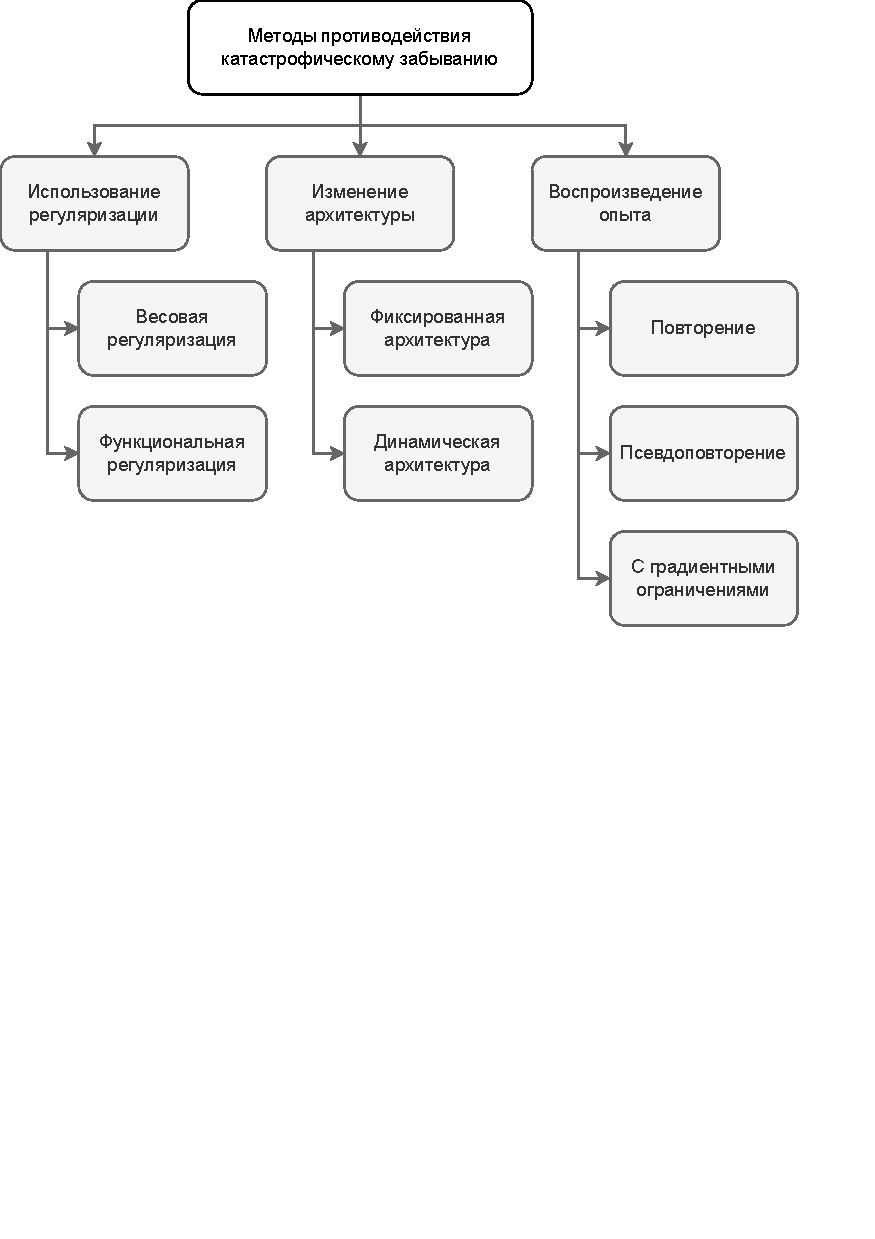
\includegraphics[width=\linewidth]{figures/taxonomy.pdf}
    \caption{Двухуровневая таксономия методов противодействия катастрофическому
        забыванию, предложенная в \cite{kumar2024methodology}. Во второй строке
        показаны три базовых подхода: использование регуляризации
        (regularization-based), изменение архитектуры (architecture-based) и
        воспроизведение опыта (replay-based). Ниже перечислены подкатегории,
        составляющие каждый из подходов.}
    \label{fig:taxonomy}
\end{figure}

Чтобы наглядно сравнить то, как свойство локальной поддержки функций активации
в KAN взаимодействует с каждой из принципиально отличающихся друг от друга
стратегий противодействия катастрофическому забыванию, было принято решение
адаптировать по одному методу из каждого подхода. Несмотря на упоминание в
литературе современных (как правило, гибридных) методов, предпочтение
отдавалось классическим алгоритмам. Они имеют прозрачную теоретическую
основу и достаточно просты для переноса в новую архитектуру, однако по-прежнему
выступают в качестве базовых моделей в большинстве современных исследований.

Оставшаяся часть главы посвящена описанию принципов, лежащих в основе выделенных
подходов, а также обзору алгоритмов, которые их реализуют.
\subsection{Подход с использованием регуляризации}
\subsubsection{Весовая регуляризация (Prior Focused)}
Основной принцип методов с весовой регуляризацией, таких как Elastic
Weight Consolidation (EWC) \cite{kirkpatrick2017overcoming} и
Synaptic Intelligence (SI) \cite{zenke2017continual}, заключается в
использовании новой функции потерь \(\mathcal{L}_{\mathrm{total}}\), полученной
добавлением в стандартную функцию потерь \(\mathcal{L}\) нового
слагаемого, штрафующего за изменение тех параметров нейронной сети, которые
имели наибольшую важность для выполнения предыдущих задач. В терминах ранее
введенных обозначений:
\begin{equation}
    \mathcal{L}_{\mathrm{total}}\bigl(f_\theta(x),y,\theta^{(t-1)}\bigr)\\
    =\mathcal{L}\bigl(f_\theta(x),y\bigr)\\
    +\bigl\lVert\theta-\theta^{(t-1)}\bigr\rVert_{\Sigma}\,,
\end{equation}
где:\\
\(\theta^{(t-1)}\) - априорные значения параметров, отклонение от которых должно
быть ограничено,\\
\(\Sigma\) - матрица оценок важности параметров с точки зрения их влияния на
качество выполнения предыдущих задач,\\
\(\lVert\cdot\rVert_{\Sigma}\) - взвешенная норма.\\
Часто используется L2-норма, с которой регуляризующее слагаемое принимает вид
\(\frac{1}{2}(\theta-\theta^{(t-1)})^T\Sigma(\theta-\theta^{(t-1)})\).
Это можно интерпретировать как наделение весов внутренним состоянием, которое
определяет уровень их пластичности. Другой полезной интерпретацией является
рассмотрение таких методов в качестве последовательного приближенного
Байесовского вывода для параметров нейронной сети.

Одним из ключевых аспектов рассматриваемых методов считается оценка важности
параметров. Распространённым подходом является использование информационной
матрицы Фишера (Fisher Information Matrix, FIM), которая показывает как
небольшие изменения параметров повлияют на значение функции потерь. Как правило,
для ускорения вычислительных процедур используется диагональная аппроксимация
FIM, что означает предположение о независимости признаков. Вторым существенным
недостатком матрицы Фишера оказалась вычислительная затратность. Вместе они
привели к появлению целого ряда методов
\cite{zenke2017continual,aljundi2018memory}, аппроксимирующих FIM или заменяющих
её прямой подсчет эвристическими методами.

В рамках данного исследования методы весовой регуляризации представляют
значительный интерес, так как отличия в способе параметризации KAN приводят к
изменению ландшафта функции потерь, а это может оказать влияние на эффективность
подхода с использованием регуляризации.

\subsubsection{Функциональная регуляризация (Data Focused)}
По аналогии с весовой регуляризацией, функциональная регуляризация добавляет
новое слагаемое в функцию потерь \(\mathcal{L}\). Однако эффективная и вместе с тем корректная
оценка весов модели представляет большую сложность из-за комплексной взаимосвязи
между поведением нейронной сети и её параметрами. Из-за этого оказывается
оправданным уход от пространства параметров к оперированию ограничениями
непосредственно в функциональном пространстве нейронной сети:
\begin{equation}
    \mathcal{L}_{\mathrm{total}}\bigl(f_\theta(x),y,\theta^{(t-1)}\bigr)\\
    =\mathcal{L}\bigl(f_\theta(x),y\bigr)\\
    +\left\langle f_\theta,f_{\theta^{(t-1)}}\right\rangle_{\mathcal{A}}\,,
\end{equation}
где:\\
\(\mathcal{A}\) - множество элементов из набора входных данных, выступающих в
роли якорных точек (anchor points),\\
\(f_{\theta^{(t-1)}}\) - отображение, сопоставляющее каждому элементу из множества
\(\mathcal{A}\) (якорных точек) соответствующий выход нейронной сети с
параметрами \(\theta^{(t-1)}\),\\ 
\(\left\langle\cdot,\cdot\right\rangle\) - мера близости на множестве
\(\mathcal{A}\).\\
Таким образом, основная цель функциональной регуляризации состоит в минимизации
различий между выходами новой \(f_\theta\) и старой \(f_{\theta^{(t-1)}}\)
нейронных сетей на множестве специальных элементов входного набора данных 
\(\mathcal{A}\), называемых якорными точками.

Существуют различные способы измерить расхождение между функциями \(f_\theta\) и
\(f_{\theta^{(t-1)}}\). Наибольшую популярность приобрёл использованный в
алгоритме Learning without Forgetting (LwF) \cite{li2016learning} подход с
дистилляцией знаний \cite{hinton2015distilling}. Поскольку расхождение между
\(f_\theta\) и \(f_{\theta^{(t-1)}}\) не обязательно измерять только в выходном
пространстве нейронной сети, в некоторых работах, например
\cite{roy2023subspace}, применяется дистилляция признаков, при которой для
передачи знаний от «учителя» к «ученику» используются не только выходы сети, но
и формируемые в скрытых слоях промежуточные представления (признаки).

Ещё одним важным вопросом в функциональной регуляризации является выбор якорных
точек \(\mathcal{A}\). Формирование этого множества путём случайного выбора
элементов из входного набора данных может оказаться достаточным лишь для
относительно простых задач. Одно из решений состоит в использовании текущей
тренировочной сессии \(B_t\) в качестве \(\mathcal{A}\), как в алгоритме LwF,
однако такой подход применим только в случае, если данные в
разных тренировочных сессиях имеют одинаковую модальность (например, являются
изображениями). Существуют подходы, стремящиеся выбрать из каждой
тренировочной сессии ограниченный набор репрезентативных в некотором смысле
обьектов, но вопрос оптимального выбора якорных точек во многом остается
открытой проблемой.

Необходимость использовать для выбора якорных точек эвристические методы,
способных внести неопределенность в результаты экспериментов из-за отличий между
архитектурами KAN и MLP, обусловили отказ от рассмотрения функциональной
регуляризации при поиске подходящих для адаптации методов.
\subsection{Подход с изменением архитектуры}
Рассмотренный ранее подход предназначен для обучения модели выполнению
нескольких задач посредством эффективного переиспользования одного и того же
набора параметров, задействованного во всех тренировочных сессиях. Однако
существует другой подход: назначение для каждой из задач обособленного
(возможно, непересекающегося) набора параметров с помощью изолирования
их друг от друга в рамках одной модели (фиксированная архитектура) или создания
новых моделей, приспособленных для решения отдельных задач (динамическая
архитектура). Это позволяет избегать перезаписи информации, содержащейся в
параметрах нейронной сети, тем самым снижая воздействие катастрофического
забывания. 
\subsubsection{Фиксированная архитектуры (Fixed Network)}
Основным принципом моделей с фиксированной архитектурой является изоляция
параметров, используемых в разных тренировочных сессиях, для уменьшения их
взаимного влияния на предварительно выученные представления. Среди
сильных сторон фиксированных сетей выделяют низкий расход памяти и относительную
простоту. Однако они требуют тщательного планирования при выделении весов под
каждую из задач, а также, как и сети с динамической архитектурой, они часто
нуждаются в информации о текущем типе задачи в условиях инкрементального
обучения задачам (task-incremental learning).

Центральным вопросом в сетях с фиксированной архитектурой является способ
разделения весов на группы: следует ли фиксировать группы заранее или позволить
им формироваться в процессе обучения; выбирать расположение весов в рамках одной
группы случайно или целыми блоками.

Одной из наиболее ранних попыток предложить ответ на эти вопросы стала
архитектура PathNet \cite{fernando2017pathnet}. В нём каждый слой заранее разбивается на \(M\)
модулей (групп нейронов), а в процессе обучения генетическим алгоритмом ищется
оптимальный маршрут (path), представляющий собой вектор индексов, указывающий,
какие из \(N<M\) модулей в каждом слое будут активны в данной задаче. Передача сигнала
происходит только между активными модулями соседних слоёв, поэтому веса
остальных нейронов не участвуют ни в прямом (forward pass), ни в обратном
(backward pass) проходе и не обновляются в ходе обратного распространения
ошибки. Считается, что априорное разбиение параметров на группы, как у PathNet,
обеспечивает высокую стабильность, но может приводить к нехватке выразительности
сети из-за фрагментации параметрического пространства

В качестве отдельного направления внутри фиксированных сетей следует выделить
архитектуру Fixed Expansion Layer (FEL) \cite{coop2013ensemble}. Её основная
идея заключается в добавлении расширенного слоя с жёстко заданными, необучаемыми
весами. Он призван разреживать проходящие через него сигналы, благодаря
чему обновление градиента в течение очередной тренировочной сессии затрагивают
лишь обособленные группы параметров предыдущего слоя, что резко снижает количество
нежелательных изменений в параметрах, ответственных за решения разных задач. 
В то же время расширенный слой остаётся фиксированным, поэтому в отличие от
методов с динамической архитектурой, рассматриваемых далее, его использование не
приводит к неограниченному росту числа параметров.

Алгоритмы с фиксированной архитектурой представляют больший интерес, чем с
динамической архитектурой, так как они направлены на локализацию изменений
параметров в отдельных группах фиксированного размера, а этот эффект может быть
усилен благодаря свойству локальности поддержки функций активации KAN.
\subsubsection{Динамическая архитектура (Dynamic Network)}
Нейронные сети с динамической архитектурой можно условно разделить на две
группы: модели, использующие ансамблевые методы, а также модели, использующие
расширение архитектуры (network expansion).

К первой группе относятся алгоритмы, стремящиеся избежать катастрофического
забывания посредством обучения нескольких моделей «экспертов» и комбинирования
их ответов. Например, Learn++ \cite{polikar2001learn} адаптирует классический
алгоритм AdaBoost, наращивая ансамбль после каждой тренировочной сессии
и делая итоговое предсказание с помощью взвешенного голосования. Недостатком
Learn++ является линейный рост требуемой для хранения весов памяти и
увеличение времени инференса. Развитие этого подхода было предложено в
\cite{ren2017lifelong}, где вводится весовая схема, способная одновременно как
добавлять, так и исключать экспертов в зависимости от их полезности в последних
тренировочных сессиях. Особое место среди трудностей, возникающих при разработке
методов, представляющих собой ансамбль экспертов, занимает необходимость выбора
эксперта для получения предсказания.

В свою очередь, модели, использующие расширение архитектуры, в каждой
тренировочной сессии добавляют в изначальную архитектуру новые нейроны или целые
слои, а параметры, отвечающие за ранее выученные задачи, замораживают. Такой
приём подавляет катастрофическое забывание, однако, как и в случае с предыдущей
группой, приводит к линейному росту объёма памяти и вычислительных издержек.
Ранние методы, такие как PNN \cite{rusu2016progressive}, имели простой принцип,
интегрируя в архитектуру новые цепочки нейронов (нейронные сети единичной
ширины), фиксируя веса предыдущих столбцов и обучая новые веса переиспользовать
полезные признаки, сформировавшиеся в течение предыдущих тренировочных сессий.
Такие методы имели типичную для моделей с динамической архитектурой проблему с
линейным ростом затрачиваемых ресурсов и требовали выбора правильных столбцов 
для получения предсказаний. Результатом дальнейших исследований стал гибридный
метод Progress \& Compress (P \& C) \cite{schwarz2018progress}, объединивший в
себе методы PNN и EWC и добившийся работы с использованием постоянного объема
памяти.

Так как используемые в классических алгоритмах с динамической архитектурой
ансамблирование и расширение архитектуры не учитывают особенности структуры
базовой модели, их адаптация для KAN не предоставит новой информации. В свою
очередь, современные методы, например P \& C, слишком сложны, чтобы их
адаптировать. Поэтому было принято решение отказаться от дальнейшего 
рассмотрения методов из этой категории.
\subsection{Подход с воспроизведением опыта}
\subsubsection{Повторение (Rehearsal)}
Главный принцип методов с повторением заключается в сохранении небольшого
подмножества элементов предыдущих тренировочных сессий и периодическом
включении их в текущую выборку данных. Классическим примером, реализующим этот
принцип является алгоритм Experience Replay (ER) \cite{rolnick2019experience}.
Для повышения репрезентативности сохраняемых экземпляров, в случае
инкрементального обучения классам, стремятся выбирать из тренировочных сессий
такие примеры, которые наиболее близки к среднему представлению класса в
признаковом пространстве. В других задачах непрерывного обучения отбор
репрезентативных объектов может оказаться затруднителен.

Известным примером архитектуры с повторением является GeppNet
\cite{gepperth2016bioinspired}, которая реализует отбор репрезентативных
объектов через использование самоорганизующейся карты (self-organising map, SOM),
выступающей в роли буфера долгосрочной памяти и организующая входные векторы на
двумерной решётке с сохранением топологии исходного распределения.

Как правило, методы с повторением оказываются очень эффективны и сравнительно
просты в реализации, однако их серьёзным недостатком является хранение реальных
примеров, которое предполагает линейный рост объема необходимой памяти и может
нарушать требования безопасности при обработке конфиденциальных данных.

В данной работе, по причине высокой популярности и эффективности, методам с
повторением отдавалось наибольшее предпочтение, в частности, благодаря
существованию алгоритмов, совмещающих вышеописанные свойства с автоматическим
формированием буфера памяти.
\subsubsection{Псевдоповторение (Pseudo Rehearsal)}
В основе идеи псевдоповторения лежит воспроизведение искусственных примеров
из предыдущих тренировочных сессий, полученных с помощью генеративных
моделей. Затем эти примеры объединяются с текущим набором данных в
процессе обучения, что позволяет избежать явного хранения реальных образцов.

Искусственные примеры и соответствующие метки создается посредством пропускания
случайного шума через отдельную генеративную модель (например, GAN), но с ростом
сложности генерация репрезентативных образцов может оказаться чрезвычайно
трудной задачей. Такие псевдо-образцы часто не полностью отражают истинное
распределение прошлых данных, поэтому отдельным направлением исследований
является поиск способов сохранения способности генераторов синтезировать
репрезентативные примеры. Кроме того, их качественно обучение и поддержка
требуют значительных ресурсов и времени, что не всегда реализуемо на практике.

Таким образом, основное преимущество методов с псевдоповторением (pseudo
rehearsal) перед методами с повторением (rehearsal) сводится к отсутствию
необходимости хранения реальных данных, а значит, снижению требований к
объему памяти и повышению безопасности при работе с чувствительными данными.
Взамен появляется необходимость обучения отдельной генеративной нейронной сети,
которая сама по себе будет подвержена катастрофическому забыванию и потребует
использования регуляризации или других методов предотвращения появления смещений
в её априорном распределении.

То, что генеративных нейронные сетей, используемые в составе методов с
псевдоповторением, требуют больших вычислительных ресурсов, а также то, что
генератор сам подвержен забыванию, что усложняет эксперименты, стало причиной
для отказа от их дальнейшего рассмотрения в рамках данного исследования.
\subsubsection{С градиентными ограничениями (Constrained)}
Методы с градиентными ограничениями также сохраняют в буфер подмножество примеров
из предыдущих задач и используют их для вычисления градиента функции потерь на
этих примерах при обучении на новой задаче. Если градиент в текущей
тренировочной сессии конфликтует с градиентами буфера (то есть их скалярное
произведение отрицательно), выполняется проекция нового градиента на выпуклую
область, образованную этими градиентами, чтобы не избежать потери
производительности в предыдущих задачах.

Наибольшую популярность среди constrained-методов приобрёл алгоритм Averaged
Gradient Episodic Memory (A-GEM). В нём для ускорения вычислительной процедуры
вместо градиентов функции потерь по каждому из содержащихся в буфере образцов
используется усреднённый градиент буфера. Если градиент текущей задачи
конфликтует с этим усреднённым градиентом, то градиент текущей задачи
проецируется на гиперплоскость, ортогональную градиенту из буфера. 

К преимуществам методов с градиентными ограничениями можно отнести архитектурную
простоту и возможность выбора между формальными гарантиями невозрастания потерь
на прошлых задачах (при вычислении градиентов по каждому из примеров в
буфере памяти) и высокой производительности (при использовании упрощённых
вариантов по типу A-GEM). Недостатки обсусловлены главным образом наличием
буфера памяти: требуется линейное по числу тренировочных сессий
количество ресурсов, имеются проблемы с конфиденциальностью и необходимо решать,
какие примеры хранить в памяти, чтобы содержание буфера было репрезентативным. 

В целом, свойства методов из рассматриваемой категории схожи с таковыми у
методов с повторением. Однако в отличие от них, методы с градиентными
ограничениями разделены на две группы. Первая (вычисление всех градиентов в
буфере памяти) сложна в реализации и вычислительно затратна, а вторая (вычисление
усреднённого градиента) из-за упрощённой процедуры вычисления градиентов может
затруднить анализ результатов экспериментов. Обе эти группы недостаточно
универсальны, так что окончательный выбор пал на методы с повторением.
\pagebreak



\section{Построение усовершенствованных моделей на базе архитектуры KAN}
\label{chap:improvedmodelsbuilding}
Для достижения целей, сформулированных в настоящем исследовании, в первую
очередь потребовалась программная реализация нейронной сети Колмогорова–Арнольда.
Как и MLP, KAN - это многослойная полносвязная нейронная сеть, состоящая из
нейронов, граней и функций активации. Наглядное сравнение между этими
архитектурами приведено на рисунке \ref{fig:kan_vs_mlp}. Их главным отличие
заключается в том, что в KAN функции активации перемещены с нейронов на грани и
являются обучаемыми.  Строение одного слоя KAN изображено на рисунке
\ref{fig:kanlayer}. Если обозначить вход слоя как \(x\in\mathbb{R}^{n_x}\) и
выход как \(y\in\mathbb{R}^{n_y}\), где \(n_x\) и \(n_y\) - соответствующие
размерности, то слой \(\Phi\) можно задать матрицей функций:
\begin{equation}
    \Phi=\left[\phi_{j,i}\right]_{j=1,\dots,n_y}^{i=1,\dots,n_x},
\end{equation}
где каждая \(\phi_{j,i}:\mathbb{R}\to\mathbb{R}\) - независимая обучаемая
скалярная функция. Тогда вычисление выходных значений слоя - это просто
суммирование:
\begin{equation}
    y=\Phi\cdot x,\quad y_j=\sum_{i=1}^{n_x}\phi_{j,i}(x_i).
\end{equation}
\begin{figure}[ht]
    \centering
    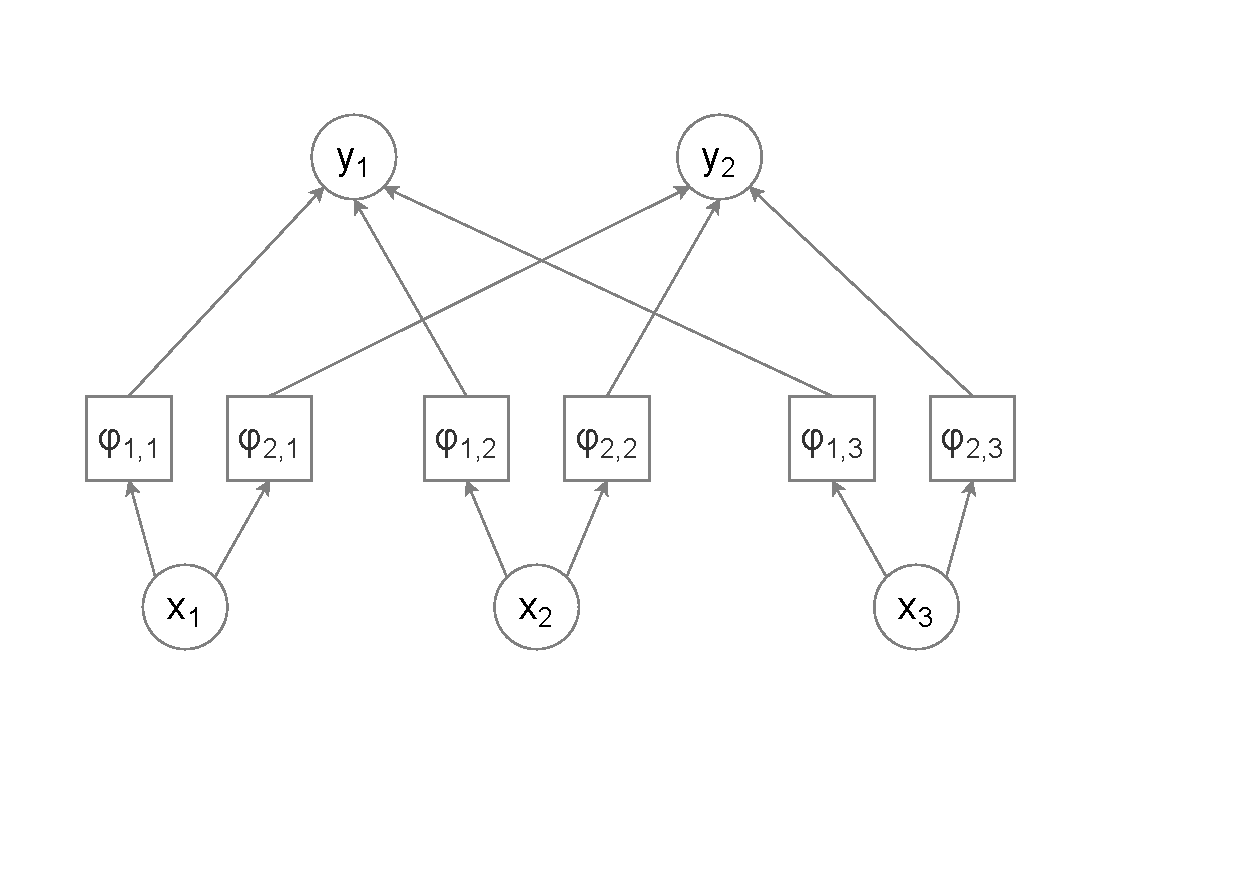
\includegraphics[width=\linewidth]{figures/kanlayer.pdf}
    \caption{Схематическое изображение одного слоя \(\Phi\) нейронной сети
        Колмогорова-Арнольда}
    \label{fig:kanlayer}
\end{figure}
Существует множество способов параметризации функций активации \(\phi_{j,i}\).
Наибольший интерес для применения в непрерывном обучении представляют формулы со
свойством локальности поддержки. Одним из таких вариантов является использование
базисных сплайнов \(B^{(k)}\) порядка \(k\). Значение функции в данной точке
вычисляется как линейная комбинация значений базисных сплайнов в этой точке с
обучаемыми коэффициентами:
\begin{equation}
    \phi_{j,i}(x)=\sum_{m=1}^kc_{j,i,m}B_m^{(k)}(x),
\end{equation}
где \(B^{(k)}_m\) - базисные функции на заранее заданной или адаптируемой
сетке (см. рисунок \ref{fig:bspline}), \(c_{j,i,m}\) - обучаемые коэффициенты.
\begin{figure}[ht]
    \centering
    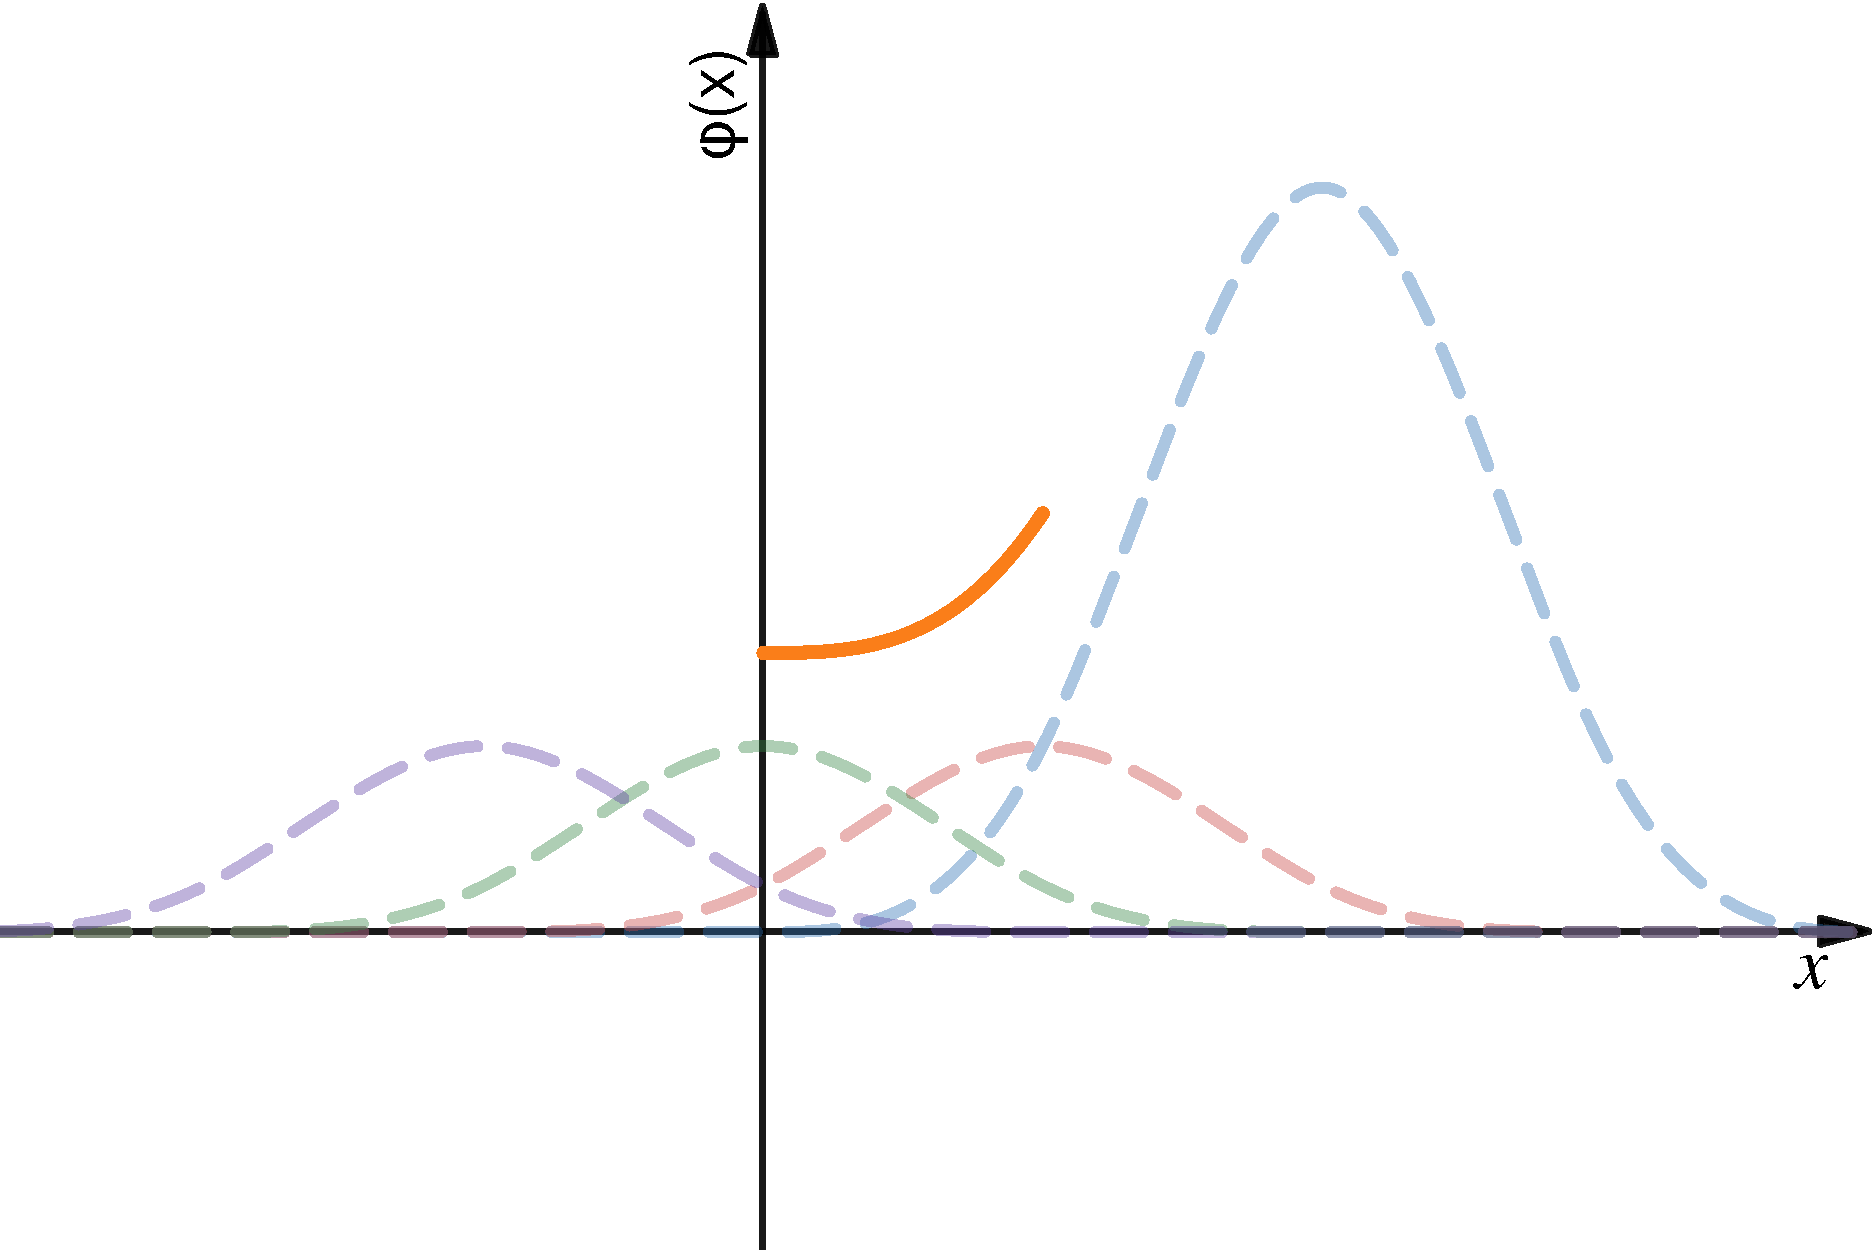
\includegraphics[width=\linewidth]{figures/bspline.pdf}
    \caption{Пример функции активации \(\phi:[0,1]\to\mathbb{R}\) (оранжевая
    сплошная кривая), параметризованной с помощью линейной комбинации четырех
    базисных сплайнов с коэффициентами 1,1,1,4 (разноцветные пунктирные кривые).}
    \label{fig:bspline}
\end{figure}
В официальной программной реализации KAN к значению сплайна в функции активации
добавляют дополнительное слагаемое - нелинейную функцию \(b\) (по-умолчанию
SiLU) и используют масштабирующие коэффициенты \(s_b\) и \(s_s\):
\begin{equation}
    \phi_{j,i}(x)=s_bb(x)+s_s\sum_{m=1}^kc_{j,i,m}B_m^{(k)}(x),
\end{equation}
что по заявлениям разработчиков улучшает начальную стабильность обучения.

Из-за внесения этих изменений в архитектуру, официальная программная реализация
KAN \cite{pykan}, как показано в \cite{yu2024kan}, полностью утратила
способности к сохранению информации в условиях непрерывного обучения и не могла
быть использована в настоящем исследовании. По этой причине была разработана
самостоятельная программная реализация сетей Колмогорова–Арнольда, имеющая ряд
отличий от версии, предложенной в оригинальной научной публикации.
\paragraph{Ключевые отличия реализации}
\begin{enumerate}
    \item \textbf{B-сплайны фиксированного порядка}. Поскольку
        вычисление значения базисного сплайна произвольного порядка требует
        использования рекурсивного алгоритма Де Бура, было решено зафиксировать порядок
        используемых в функциях активации \(\phi_{j,i}\) B-сплайнов. Благодаря этому
        удалось вывести явную формулу для кубического базисного сплайна и векторизовать
        операции вычисления его значения.
    \item \textbf{Функций активации, состоящие только из линейной комбинации
        базисных сплайнов}. Масштабирующие коэффициенты \(s_b\) и \(s_s\) в 
        условиях непрерывного обучения неизбежно оказываются общими параметрами для всех
        задач, так как изменяют значение функции активации во всех точках одновременно. 
        Поэтому их оптимизация в текущей тренировочной сессии фактически обесценивает
        представления, содержащие в себе информацию о предыдущих задачах.
    \item \textbf{Фиксированная сетка базисных функций вкупе, общая
        пакетная нормализация (Shared Batch Normalization) и ограничение области входных
        значений}. Как следует из \cite{lee2025kolmogorov}, оригинальный подход, 
        подразумевающий адаптацию сетки базисных функций по мере появления новых
        объектов не может быть использован в непрерывном обучении. Вместо этого ко
        входным векторам применяется слой пакетной нормализации, а затем
        область входных значений ограничивается на отрезке \([0,1]\).
    \item \textbf{Процедура инициализации параметров}, адаптированная из
        \cite{efficientkan}. Сначала для каждой функции
        активации в нейронной сети формируется равномерная сетка узлов \(G\)
        размером \(|G|\). Затем для каждого узла генерируется целевое значение
        \(B\sim N\!\left(0,\sigma^{2}\right)\), где
        \(\sigma=\dfrac{1}{10(|G|-3)}\). После этого коэффициенты базисных
        сплайнов (параметры модели) \(C\) вычисляются решением задачи наименьших
        квадратов \(AC=B\), где \(A\) - начальные значения функций активации в
        узлах равномерной сетки. Такой подход обеспечивает интерполяцию функций
        активации через заданные в узлах значения
\end{enumerate}
Исходный код программной реализации KAN, использованной в настоящем исследовании,
приведён в приложении \ref{apdx:kan}. Помимо этого, весь исходный код доступен
в открытом репозитории \cite{spbubachelorthesis}.
\subsection{Подход с использованием регуляризации}
Среди методов противодействия катастрофическому забыванию, реализующих подход с
использованием регуляризации, с целью адаптации для KAN был выбран EWC,
который, согласно таксономии из главы \ref{chap:analysisofexistingapproaches},
относится к подкатегории методов с весовой регуляризацией.

В KAN каждая обучаемая функция активации \(\phi_{j,i}\) параметризуется
коэффициентами кубических B-сплайнов
\(\{c_{j,i,m}\}_{m=1}^{k}\), обладающих локальной поддержкой.
Следовательно, изменение отдельного коэффициента влияет лишь на
ограниченный диапазон входных значений, что уменьшает перекрытие между
представлениями, относящимся к разным задачам. Регуляризация
\(\theta=\{c_{j,i,m}\}\) должна усилить локальный характер обновлений и подавить
избыточные глобальные сдвиги, приводящие к катастрофическому забыванию в
оригинальной реализации KAN.

Основная идея EWC заключается во включении в стандартную функцию потерь
\(\mathcal{L}\) дополнительного регуляризирующего слагаемого,
штрафующего отклонение параметров \(\theta\) от значений \(\theta^{(t-1)}\),
полученных после предыдущей тренировочной сессии \(t-1\):
\begin{equation}
    \mathcal{L}_{\mathrm{EWC}}\bigl(f_\theta(x),y\bigr)\\
    =\mathcal{L}\bigl(f_\theta(x),y\bigr)\\
    +\frac{\lambda}{2}\sum_{i}F^{(t-1)}_{i}(\theta_{i}-\theta^{\star}_{i})^{2},
\end{equation}
где \(\lambda\) — гиперпараметр, определяющий силу регуляризации, а
\(F^{(t-1)}\)— диагональная аппроксимация информационной матрицы Фишера,
служащая оценкой важности каждого параметра для задач, выученных ранее.  
В классической постановке для каждой задачи хранится собственная
\(\theta^{\star}\) и своя \(F\), но такое решение требует большого объёма памяти,
что непрактично при большом числе сессий.

Поэтому в настоящей работе реализована модификация оригинального метода под
названием online EWC \cite{schwarz2018progress}, где используется единая матрица
Фишера \(F^{(t)}\) для всех задач, обновляемая по правилу экспоненциального
сглаживания:
\begin{equation}
    F^{(t)}_i=\gamma\,F^{(t-1)}_i+(1-\gamma)\,\hat F^{(t)}_i,\qquad
    0<\gamma<1,
\end{equation}
где \(\hat F^{(t)}\) — свежая оценка Фишера на данных текущей
сессии, а \(\gamma\) — коэффициент затухания.  
Благодаря этому объём дополнительной памяти становится фиксированным, но регуляризация
постепенно «забывает» статистику давно прошедших задач.

Расчёт оценки матрицы Фишера \(\hat F^{(t)}\) производится на данных текущей
тренировочной сесии \(B_t\) размером \(N_t\):
\begin{equation}
    \hat F^{(t)}_i=\frac{1}{N_t}\sum_{(x,y)\in B_t}
        \left(
        \frac{\partial\mathcal{L}}{\partial\theta_i}
        \Big|_{(x,y)}
        \right)^2,
    \label{eq:fisher_batch}
\end{equation}
по-умолчанию реализовано взятие градиента именно по модельным предсказаниям
(expected Fisher), а не по истинным меткам классов (empirical Fisher). В
программной реализации присутствуют обе версии, но в статье 
\cite{kunstner2019limitations} использование эмпирической матрицы Фишера было
подвержено критике.
\paragraph{Ключевые отличия реализации}
\begin{enumerate}
    \item \textbf{Онлайн-обновление}. Вместо хранения набора пар \((\theta^{\star},F)\)
        для всех
        завершённых задач поддерживается единственный вектор \(F^{(t)}\) и
        набор параметров \(\theta^{\star}\), перезаписываемые после каждой
        тренировочной сессии. Это снижает требование к памяти и ускоряет доступ к
        статистике.
    \item \textbf{Адаптивная оценка меток}.  
        Флаг \texttt{empirical\_estimate} позволяет подменять
        истинные метки \(y\) предсказаниями модели
        \(\arg\max f_{\theta}(x_b)\), что
        позволяет выбирать между вычислением эмпирической и ожидаемой
        матрицами Фишера.
\end{enumerate}

Программный реализация функции потерь EWCLoss приведён в
приложении \ref{apdx:regularized_kan}.
\subsection{Подход с изменением архитектуры}
Среди методов противодействия катастрофическому забыванию, реализующих подход с
изменением архитектуры, с целью адаптации для KAN был выбран FEL, который,
согласно таксономии из главы \ref{chap:analysisofexistingapproaches}, относится
к подкатегории методов с фиксированной архитектурой.

Метод FEL расширяет каждое скрытое пространство нейронной сети в \(r\) раз за счёт
случайно зафиксированных весов \(W\!\in\!\mathbb{R}^{kd\times d}\). Благодаря
этому представления прежних задач проецируются в более разрежённое пространство,
где их легче изолировать от новых данных и тем самым снизить воздействие
катастрофического забывания. В приведённой реализации при прямом проходе для
входного вектора \(x\!\in\!\mathbb{R}^{d}\) вычисляются выходные значения
\(Wx\), центрированные с помощью нормализации по слоям \(\operatorname{LayerNorm}\):
\begin{equation}
    z=\operatorname{LayerNorm}(Wx),
\end{equation}
а затем эти значения разреживаются с помощью
бинарной маски \(m(x)\!\in\!\{0,1\}^{rd}\), пропускающей только несколько наибольших по модулю
компонент \(z\) и зануляющей остальные значения выходного слоя.

В отличие от онлайн-FEL, где входы обрабатываются по одному,
реализация использует батч-умножение $Wx$ и выполняет
$k$-WTA \emph{для каждого} примера батча, сохраняя
асимметрию градиентов между разными задачами.
Поскольку $W$ не обучается, вычислительная стоимость FEL
ограничивается одной матрицей умножения и сортировкой по столбцам.
\paragraph{Ключевые отличия реализации}
\begin{enumerate}
    \item \textbf{Инициализация.}  
        Ненулевые элементы \(W\) инициализируются распределением 
        \(\mathcal{N}(0,2/n_\text{in})\) (Kaiming initialization), как
        рекомендовано для необучаемых слоёв глубоких нейронных сетей.
    \item \textbf{Нормализация}  
        Используется LayerNorm с параметрами \(\gamma\!=\!1,\beta\!=\!0\),
        чтобы стандартизировать масштаб выходных значений без использования
        глобальных обучаемых коэффициентов, которые могли бы приводить к
        массовому обновлению весов.
    \item \textbf{Батч-умножение \(Wx\)}. В отличие от оригинальной версии FEL,
        
\end{enumerate}

Исходный код классов FELLayer и ArchitecturalKAN приведён в приложении
\ref{apdx:architectural_kan}.
\subsection{Подход с воспроизведением опыта}
Среди методов противодействия катастрофическому забыванию, реализующих подход с
воспроизведением опыта, с целью адаптации для KAN был выбран GeppNet, который,
согласно таксономии из главы \ref{chap:analysisofexistingapproaches}, относится
к подкатегории методов с повторением.

В основе алгоритма GeppNet лежит самоорганизующаяся карта
(Self-Organizing Map, SOM), служащая «буфером долговременной памяти», —
она проецирует входные векторы \(x\!\in\!\mathbb{R}^{d}\) на
двумерную решётку прототипов \(W=\{\,w_{j}\in\mathbb{R}^{d}\,\}_{j=1}^{M}\) и
тем самым автоматические структурирует поток входных данных без сохранения
отдельных примеров.
Для получения предсказаний активность каждого прототипа рассчитывается как
\begin{equation}
    s_{j}(x)=
    \exp\!\Bigl(-\tfrac{\lVert x-w_{j}\rVert^{2}}{2\sigma_{\text{in}}^{2}}\Bigr),
    \qquad
    j=1,\dots ,M,
    \label{eq:som_similarity}
\end{equation}
где \(\sigma_{\text{in}}\) — дисперсия в пространстве признаков. Полученный
вектор \(s(x)\in\mathbb{R}^{M}\) используется в качестве входных данных для
следующего слоя. В классическом GeppNet это MLP, а в настоящей работе - слой KAN.

В оригинальном GeppNet прототипы обновляются после каждой выборки в режиме
online-обучения, что делает невозможным оптимизацию вычислительных процедур,
поэтому вместо обычной SOM была реализована её модификация - Batch-SOM
\cite{cheng1997convergence}. Для батча \(X=\{x_{i}\}_{i=1}^{B}\) ищутся
ближайшие прототипы в пространстве признаков (best matching units, BMU):
\begin{equation}
    \mathrm{bmu}(x)=\underset{j}{\arg\min}\lVert x-w_j\rVert,
\end{equation}
после чего происходит обновлением прототипов:
\begin{equation}
    w_{j}=\frac{\sum_{i=1}^{B}h_{j,\mathrm{bmu}(x_{i})}\,x_{i}}{\sum_{i=1}^{B}h_{j,\mathrm{bmu}(x_{i})}},\\
    \qquad h_{j,k}=\exp\!\Bigl(-\tfrac{\lVert c_{j}-c_{k}\rVert^{2}}{2\sigma_{\text{grid}}^{2}}\Bigr),
    \label{eq:batch_som_update}
\end{equation}
где \(c_{j}\in\mathbb{R}^{2}\) — координаты прототипа \(w_{j}\) на квадратной
решётке, а \(\sigma_{\text{grid}}\) — дисперсия в пространстве координат.  
\paragraph{Ключевые отличия реализации}
\begin{enumerate}
    \item \textbf{Инициализация прототипов.}  
        Перед началом применения SOM проходит через одну эпоху обучения на
        базовом подмножестве данных, чтобы адаптировать под данные стартовое
        расположение \(W\), а также ускорить дальнейшее упорядочивание прототипов.
    \item \textbf{Раздельное обучение SOM и KAN}.  
        Поскольку слой KAN принимает градиенты от $\mathcal{L}$, а SOM обновляется
        отдельно, процедура обучения чередует оптимизацию KAN-классификатора
        и обновление прототипов, что не требует изменения стандартного алгоритма
        обучения.
\end{enumerate}

Программная реализация классов Rehearsal KAN и SOMLayer приведена в приложении
\ref{apdx:rehearsal_kan}.
\pagebreak




\section{Применение усовершенствованных моделей в задачах непрерывного обучения}
\begin{table}[h!]
    \begin{center}
        \begin{tabular}{ |c|c|  }
            \hline
            \multicolumn{2}{|c|}{CUB-200-2011} \\
            \hline
            Объект выборки & RGB изображение \\
            \hline
            Количество классов & 200 \\
            \hline
            Количество признаков & 2,048 \\
            \hline
            Размер обучающей выборки & 5,994 \\
            \hline
            Размер тестовой выборки & 5,794 \\
            \hline
            Тренировочные объекты/класс & 29-30 \\
            \hline
            Тестовые объекты/класс & 11-30 \\
            \hline
        \end{tabular}
        \caption{Описание используемого набора данных}
        \label{tab:dataset}
    \end{center}
\end{table}
В качестве набора данных используется CUB-200-2011 (\hyperref[tab:dataset]{Таблица 1}), содержащий в себе привычное для прикладных задач количество 
объектов и классов. Поскольку основная цель исследования - оценка эффективности 
противодействия моделей катастрофическому забыванию, а не сравнение качества 
векторных представлений объектов обучающей выборки, в качестве входных признаков
используются векторные представления, полученные из предпоследнего слоя
предобученной модели ResNet-50.

Согласно общепринятым рекомендациям, проводится несколько экспериментов:
\begin{enumerate}
    \item Обучение с перестановкой признаков.
    \item Инкрементальное обучение классам.
\end{enumerate}
Первый эксперимент оценивает способность модели сохранять несколько 
представлений одного и того же набора данных, обучаясь на них последовательно.
Второй эксперимент направлен на изучение способности модели обучаться новым 
классам данных, не забывая при этом ранее изученные классы.

Для программной реализации экспериментов использовались вспомогательные функции
и классы на языке Python, приведённые в Github репозитории
\cite{spbubachelorthesis} в следующих файлах:\\
\texttt{spbu-bachelor-thesis/spbu\_bachelor\_thesis/train\_test.py},\\
\texttt{spbu-bachelor-thesis/spbu\_bachelor\_thesis/metrics.py},\\
\texttt{spbu-bachelor-thesis/spbu\_bachelor\_thesis/datasets.py},\\
\texttt{spbu-bachelor-thesis/spbu\_bachelor\_thesis/visualization.py}.\\
Программная реализация экспериментов находится там же, в файлах\\
\texttt{spbu-bachelor-thesis/notebooks/01\_data\_preparation.py},\\
\texttt{spbu-bachelor-thesis/notebooks/02\_proposed\_models.py},\\
\texttt{spbu-bachelor-thesis/notebooks/03\_continual\_learning.py},\\
\texttt{spbu-bachelor-thesis/notebooks/04\_report\_preparation.py}.
\subsection{Обучение с перестановкой признаков}
В каждой из \(S\) тренировочных сессий (по-умолчанию \(S=4\)) к обучающей и
тестовой выборкам применялось новое случайное переставление индексов
признакового вектора. Таким образом, модель должна поочерёдно выучить \(S\)
взаимно независимых представлений одного и того же распределения без
катастрофического забывания. В каждой тренировочной сессии данные подавались
батчами по 256 примеров. Оптимизация весов нейронных сетей производилась с
помощью алгоритма NAdam до тех пор, пока метрика Mean Per Class Accuracy не
улучшалась в течение 10 эпох.

Графики с результатами проведения эксперимента над усовершенствованными моделями
находятся в приложениях
\subsection{Инкрементальное обучение классам}
Тренировочные сессии в этом эксперименте формировались путем использования
разных классов в обучающей выборке. Функция случайным образом разбивает 200
классов из набора данных CUB-200 на непересекающиеся множества: базовая
тренировочная сессия включает \(C_{\text{base}}\) классов, а каждая последующая
содержит фиксированное число \(C_{\text{inc}}\) классов. В коде по-умолчанию
\(C_{\text{base}}\gg C_{\text{inc}}\), что отражает сценарий, когда исходная
система уже обучена на крупном подмножестве данных из рассматриваемой
предметной области.

На шаге \(t\) модель обучается только на образцах последних
\(C_{\text{inc}}\) классов, тогда как тестирование проводилось на объединении
всех классов, встречавшихся на всех предыдущих шагах до \(t\) включительно.
Такой протокол соответствует задаче task-agnostic continual learning, когда
идентификатор задачи на этапе получения предсказания неизвестен.

Цикл обучения аналогичен тому, что был использован в предыдущем эксперименте:
обучение производится с ранней остановкой на основании значений метрики Mean Per
Class Accuracy.

Графики с результатами проведения эксперимента находятся в приложениях
\pagebreak




\section{Анализ экспериментов}
\pagebreak




\specialsection{Выводы}
\pagebreak




\specialsection{Заключение}
\pagebreak




\printbibliography[heading=bibintoc]
\pagebreak



\appendix
\specialsection{Приложения}
\captionsetup[listing]{name=Приложение}
\section{Исходный код усовершенствованных нейронных сетей}
\begin{center}
    % KAN
    \captionof{listing}{Исходный код на Python для модели на основе архитектуры
        KAN}
    \label{apdx:kan}
    \inputminted{python}{../../spbu_bachelor_thesis/nn/kan.py}

    % Architectural KAN
    \captionof{listing}{Исходный код на Python для усовершенствованной модели,
        реализующей подход с изменением архитектуры}
    \label{apdx:architectural_kan}
    \inputminted{python}{../../spbu_bachelor_thesis/nn/architectural_kan.py}

    % Regularized KAN
    \captionof{listing}{Исходный код на Python для усовершенствованной модели,
        реализующей подход с использованием регуляризации}
    \label{apdx:regularized_kan}
    \inputminted{python}{../../spbu_bachelor_thesis/nn/regularized_kan.py}

    % Rehearsal KAN
    \captionof{listing}{Исходный код на Python для усовершенствованной модели,
        реализующей подход с воспроизведением опыта}
    \label{apdx:rehearsal_kan}
    \inputminted{python}{../../spbu_bachelor_thesis/nn/rehearsal_kan.py}
\end{center}
\section{Графики с результатами обучения с перестановкой признаков}
\section{Графики с результатами инкрементального обучения классам}

\end{document}